% =========================================================
\section{实验设计}
\label{sec:experiments}
% =========================================================

\subsection{时序运维基准}
\label{sec:dataset}

我们构建了一个语义基准，用于受控评估动态运维场景中的时序证据检索。该数据集以公开资料中的背景信息作为约束，并借助 AI 辅助构建；它并非来源于真实电站故障日志，也不是由领域专家人工标注的真实运维数据集。公开产品文档和研究数据集主要用于约束电芯类型、典型物理范围和采样背景，而具体的运维事件过程、诊断变化、规程上下文与查询任务则通过受控的合成构建流程生成。这样的设计使我们能够有意识地引入晚到记录、版本替代、跨来源互补证据、多事件片段歧义以及持续不确定性，并比较不同检索方法对这些因素的处理能力。

整体基准构建流程如图~\ref{fig:benchmark_design} 所示。公开资料首先用于约束物理与采样背景；随后在这些约束下构造合成运维事件链，再从事件链中派生可检索证据记录和不同任务查询。对于每个查询，我们分别构建用于检索评估的参考证据流，以及用于生成评估的结构化参考答案。

\begin{figure*}[t]
    \centering
    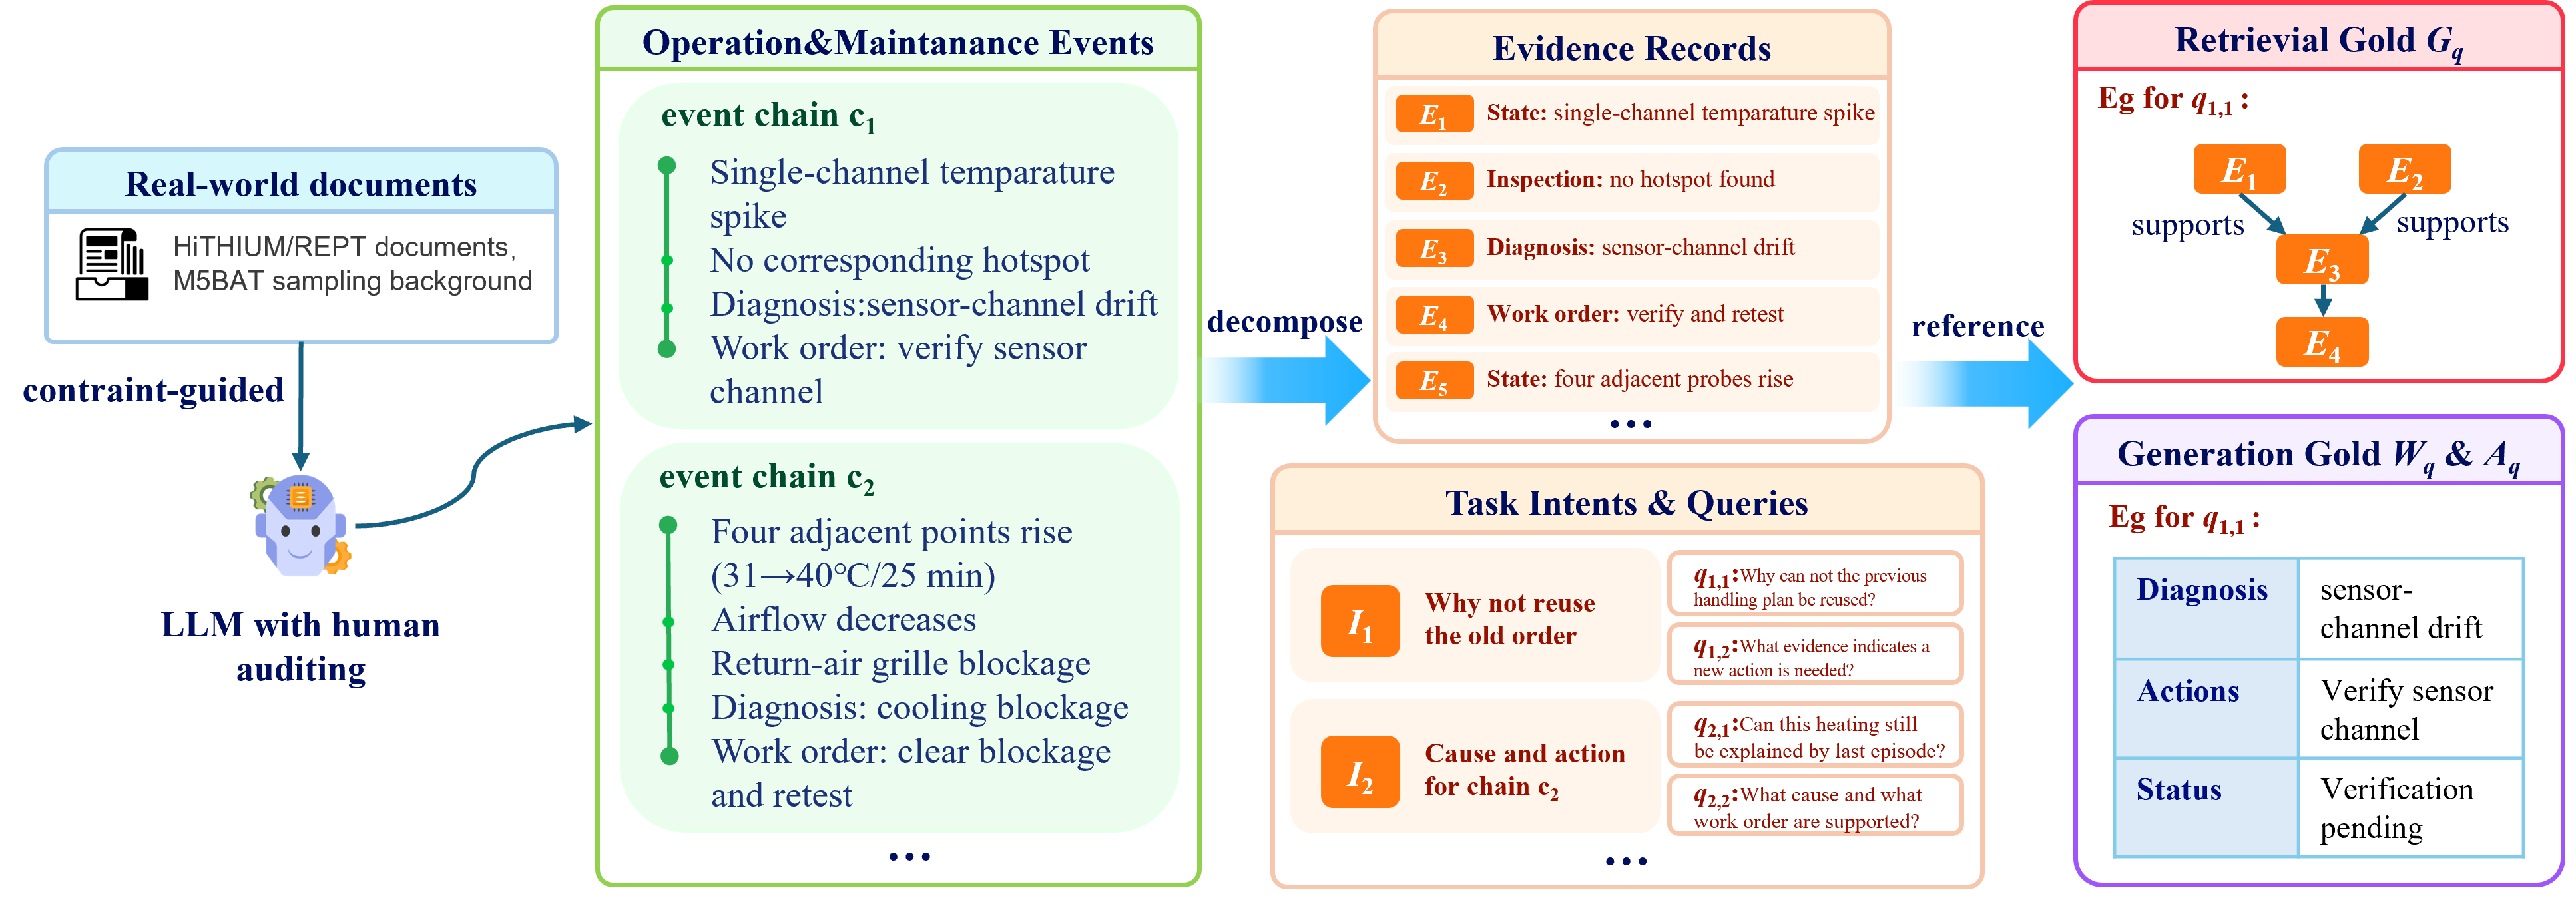
\includegraphics[width=0.98\textwidth]{figures/benchmark_design.png}
    \caption{TEF-RAG v6 Semantic Benchmark v1 的构建流程与示例。公开资料用于约束设备与数据背景；随后构造一条运维事件链 $c$，并由其派生证据记录 $e_i$、任务意图 $I_j$ 与查询 $q_{j,p}$。之后为每个查询分别构建检索参考证据流和结构化生成参考答案，用于检索与下游生成评估。}
    \label{fig:benchmark_design}
\end{figure*}

数据组织方式总结于表~\ref{tab:dataset_structure}。每条事件链表示一个完整的运维过程，并由多条可检索证据记录构成。对于每条事件链，我们构建多个不同的任务意图，每个意图再用两种措辞不同但语义相同的查询来表达。

对于每个查询，我们进一步提供一组参考标注，用于指定完成任务必须检索到哪些关键信息，以及这些证据之间应满足何种关系。因此，评估并不要求检索某一段唯一指定的文本，而是检验所检索集合是否包含足够的信息，以及这些证据能否共同构成完整的任务支撑过程。

\begin{table}[t]
\caption{基准的数据层级。}
\label{tab:dataset_structure}
\centering
\small
\begin{tabular}{@{}p{0.24\columnwidth}p{0.69\columnwidth}@{}}
\toprule
层级 & 含义 \\
\midrule
事件链 & 一个完整的运维事件过程 \\
证据 & 带有事件时间和可用时间的原子级可检索记录 \\
意图 & 定义在同一事件链上的不同运维信息需求 \\
查询 & 用不同措辞表达同一意图的查询 \\
参考证据流 & 关键证据要求及其关系约束 \\
\bottomrule
\end{tabular}
\end{table}

完整基准包含 400 条运维事件链、3,888 条证据记录、1,200 个任务意图和 2,400 条查询，共涉及 100 个目标资产。开发集、验证集和测试集均按完整事件链进行划分；由同一条事件链派生的全部查询只会出现在一个数据划分中，从而避免同一事件内容通过不同措辞同时出现在训练数据和测试数据中。

为了同时评估普通条件与特意设计的困难时序条件下的检索性能，我们将 400 条事件链平均划分为两个难度层。标准子集包含相对常见的时间与运维条件组合；temporal-hard 子集则提高了晚到证据、版本替代、多事件片段歧义、跨来源互补证据以及持续不确定性等情况的出现频率。

\begin{table*}[t]
\caption{TEF-RAG v6 Semantic Benchmark v1 的规模与数据划分。}
\label{tab:dataset_stats}
\centering
\small
\begin{tabular}{lrrrr}
\toprule
统计项 & 开发集 & 验证集 & 测试集 & 总计 \\
\midrule
构建的事件链 & 240 & 80 & 80 & 400 \\
主要任务意图 & 720 & 240 & 240 & 1200 \\
查询条目 & 1440 & 480 & 480 & 2400 \\
证据记录 & 2335 & 779 & 774 & 3888 \\
\bottomrule
\end{tabular}
\end{table*}

公开资料仅用于约束电芯类型、典型运行范围和时间采样背景，其中包括 HiTHIUM 与 REPT BATTERO 的储能电芯资料，以及 RWTH M5BAT 数据集~\cite{hithium2023v11,hithium2024v33,rept2025,rwth2026m5bat}。这些资料并不用于定义本基准中的合成故障频率、电站级阈值或具体维护因果叙事。

\subsection{结构化生成评估}

为了评估检索上下文如何反映到下游生成结果中，我们在同一组运维事件链上构建结构化参考答案。这些参考答案借助 AI 辅助生成，并经过针对所构造事件链与规定输出格式的多轮一致性检查后定稿。

每个任务意图对应一个结构化参考答案。由于同一意图下的两条查询只是在措辞上不同，而所要求的诊断、动作与验证信息相同，因此二者共享同一参考答案。开发集、验证集和测试集分别包含 720、240 和 240 个结构化参考答案，对应 1,440、480 和 480 条查询。每个输出由两部分组成：标准化工单和动作计划。工单描述诊断、推荐动作、适用规程、验证/不确定性状态以及证据引用；动作计划由原子动作及其依赖关系构成。

\subsection{基线方法}
\label{sec:baselines}

为减少检索策略之外的差异造成的混杂因素，所有方法首先都在查询时刻可用的同一证据集合上运行。我们只保留目标资产中满足
$t_e(e)\le t_q$ 且 $t_a(e)\le t_q$ 的记录，并对规程证据施加相同的版本有效性、撤回状态和型号适用性约束。在这一共享设置下，我们比较五种方法；每种方法最终最多返回五条证据记录。

\textbf{BM25。}
我们采用标准 BM25 作为词法检索基线~\cite{robertson2009bm25}。对于每个查询，分别在合法证据集合上建立索引，固定参数为 $k_1=1.5$、$b=0.75$，并直接返回得分最高的五条证据。

\textbf{BGE Reranker。}
首先使用相同的 BM25 设置检索 Top-30 候选，然后使用 \texttt{BAAI/bge-reranker-v2-m3} 对每个 $(\text{query},\text{evidence})$ 文本对重新打分~\cite{chen2024bgem3,flagembedding2026reranker}，并选取重排序得分最高的五条记录。该基线用于检验通用语义重排序器能否弥补纯词法检索的局限。

\textbf{Temporal-BM25。}
该基线在 BM25 相关性之外显式加入时间匹配项，其排序得分为
\begin{equation}
s_{\mathrm{TBM25}}(e,q)
=
\lambda\,\widetilde{s}_{\mathrm{BM25}}(e,q)
+
(1-\lambda)\,s_{\mathrm{time}}(e,q),
\end{equation}
其中，$\widetilde{s}_{\mathrm{BM25}}$ 为归一化的 BM25 得分，$s_{\mathrm{time}}$ 用于衡量证据事件时间与查询中由年份、时间区间、前/后、当前/最新等表达所隐含目标时间之间的匹配程度。对于不存在显式时间意图的查询，时间项被设为常数，因此保持原始 BM25 排序不变。在最终测试评估之前，我们在验证集上比较 $\lambda\in\{0.25,0.50,0.75\}$，选择 $\lambda=0.25$，并在后续评估中固定该值。

\textbf{TA-RAG。}
我们采用 Lau 等人提出的 Time-Aware RAG 方法~\cite{lau2025tarag}。该方法首先将查询分解为主题与目标时间范围，随后通过时间区间过滤限制候选文档，并在时间候选集合内进行语义检索与 BGE 重排序。为了将 TA-RAG 适配到本文的离散运维事件，我们将每个事件时间 $t_e(e)$ 表示为一个长度为一秒的左闭右开区间，并以 $t_q$ 作为参考时间解释查询中的相对时间表达。此外，TA-RAG 的索引仅由满足与其他方法相同的时间和规程适用性约束的证据构建，从而防止未来记录影响检索。
除用于时间分解的语言模型被替换外，时间分解、区间过滤、Nomic embedding、FAISS 检索和 BGE 重排序流程均沿用公开实现。

\textbf{TEF-RAG。}
本文方法在同一合法证据集合上执行学习式证据对筛选、查询条件化关系图构建和非线性集合级排序，并返回整体证据流得分最高的候选集合。

\subsection{评估指标}
\label{sec:metrics}

\textbf{检索。}
Recall@5 与 nDCG@5 衡量传统检索相关性。Complete@5 衡量检索集合是否包含完成任务所需的全部关键证据类别。FlowComplete@5 进一步检查这些记录能否形成正确且相互一致的证据关系，从而构成完整的时序证据流。

\textbf{生成。}
正文报告四个主要指标：Field Macro F1（strict）、Action F1、Citation F1 和 Plan EM（strict）。它们分别衡量关键工单字段、归一化动作、claim--evidence 引用以及完整动作计划的严格匹配情况。

\subsection{消融实验设置}

为分析各组成部分的贡献，我们在 480 条验证集查询上进行了四组消融：移除学习式证据对提议、移除由关系图导出的集合特征、移除难负样本挖掘，以及移除非线性集合排序器。完整模型与所有变体均使用相同的 Top-30 搜索池、相同的送入关系判断的最大证据对数量、相同的关系判断提示词与置信度阈值，以及相同的候选集合构造过程。图特征消融仅移除由关系图导出的集合特征，并重新训练同一 RankNet；难负样本消融只保留第一轮训练；非线性排序器消融则移除学习式集合排序器，改用前序的贪心证据集合选择器。
